
%%%%%%%%%%%%%%%%%%%%%%%%%%%%%%%%%%%%%%%%%%%%%%%%%%%%%%%%%%%%%%%%%%%%%%%%%%%%
% This will help you in writing your homebook
% Remember that the character % is a comment in latex

% Divide the work you have done in each of the chapters used 
% during the lab lessons in a new chapter, as in the example below, 
% using a coherent title 


% For each chapter you can include :

%-----------------------------
% VHDL file, using the sintax:


	%\begin{listato}
	%\lstinputlisting{./exeMPLE/listato1.vhd}
	%\end{listato}

% the path to the file must be correct, obviously
% Should you have listings written in other languages the method is the 
% same, but the language set up must be changed using a different 
% setting for the command \lstset{language=VHDL} in file homebook.tex 


%-----------------------------
% figures in postcript (ps) or encapsulated postcript (eps)
% format, using the syntax:

%	\begin{figure}[h]
%	\centering
%	\includegraphics[width=9cm]{./cap1/figure1.eps}
%	\caption{Put a caption if you want (didascalia...:)))}
%	\label{put-a-label-for-referring-to-this-picture}	
%	\end{figure}

% the path to the file must be correct, obviously
% you can refer to this picture in any point of your document
% by typing the instruction:

% 	\ref{put-a-label-for-referring-to-this-picture}

% that is using the same label you put in the fiure label
% when you will run the "latex command" an automatic reference to
% this figure with the correct enumeration will be inserted


%-----------------------
% comment in text format (if you are not skilled in latex and don't want to be)
% using the sintax:

	%\begin{verbatim}
	% blablabla 
	%\end{verbatim}

% The verbatimg includes text as it is, as you could write in a normal text file 

% (BETTER) If uou want to write enhancing all the latex possibilities you 
% should add to you text a few commands in some particular cases. 
% In the following you have and example of a few chapters roughtly commented
% and written all in this file: remember that you can saparate
% each chapter in different files (this is always what a latex pro does) 
% and include them using the instruction: \input{./directoryxx/fileyy.tex}


%%%%%%%%%%%%%%%%%%%%%%%%%%%%%%%%%%%%%%%%%%%%%%%%%%%%%%%%%%%%%%%%%%%%%%%%%%%%%%%
%%%%%%%%%%%%%%%%%%%%%%%%%%%%%%%%%%%%%%%%%%%%%%%%%%%%%%%%%%%%%%%%%%%%%%%%%%%%%%%%%
%%%%%%%%%%%%%%%%%%%%%%%%%%%%%%
% Beginning of latex commands
% You can copy this in a new file (e.g. cap1/cap1.tex) and inlcude it here
% using the command : \input{./cap1/cap1.tex}


% chapter 1
\chapter{Laboratorio 1}


% include here only files for the first lesson and homeworks
% here the path to figures and VHDL should be ./cap1/

%%%%%%%%%%%%%%%%%%%%%%%%%%%%%%%%%%%%%%%%%%%%%%%%%%%%%%%%%%%
% you can organize thje report usign section -> \section{Simulating an inverter}
% or subsection -> \subsection{simulating a particular type of inverter}

%%%%%%   First section
\section{Calcolo di probabilit\`a e attivit\`a: porte logiche elementari}

Il primo esercizio consiste nel valutare le probabilit\`a e attività di quattro porte logiche elementari: NOT, AND, OR e XOR.
\\
Mentre la probabilità di uscita del gate è definita dalla funzione logica stessa, la switching activity è valutata allo stesso modo per tutti i casi, mediante la seguente formula: \\
A = 2*P1*p0

Di seguito è riportata l'analisi delle porte logiche richieste, considerando ingressi equiprobabili e scorrelati.

\begin{itemize}
\item \textbf{NOT} \\
P(Y=1) = 1-P(A=1) = 0.5 \\
A(Y) = 0.5
\item \textbf{AND} \\
P(Y=1) = P(A=1)*P(B=1) = 0.25 \\
A(Y) = 0.375
\item \textbf{OR} \\
P(Y=1) = 1-((1-P(A=1))*(1-P(B=1))) = 0.75 \\
A(Y) = 0.375
\item \textbf{XOR} \\
P(Y=1) = P(A=1)*(1-P(B=1)) + P(B=1)*(1-P(A=1)) = 0.5 \\
A(Y) = 0.5
\end{itemize} 

Simulando il test bench fornito tramite ModelSim è possibile ottenere un file riportante il numero di commutazioni di ogni segnale del circuito durante il tempo di simulazione.
Il testbench fornito sfrutta un generatore di numeri casuali per generare gli ingressi delle porte, rendendo questi ultimi equiprobabili e statisticamente indipendenti. 
In particolare, è possibile ricavare la switching activity delle uscite dividendo il numero di commutazioni per il numero di cicli di clock simulati.
Sono riportati i seguenti valori:

\begin{table}
\begin{center}
\begin{tabular}{|c|c|c|c|c|}
\hline
Tc(CLK) & Tc(INV) & Tc(AND) & Tc(OR) & Tc(XOR) \\
\hline
topolino & minni & tip & tap \\
\hline
\hline
paperino & paperina & orazio & clarabella \\
\hline
qui & quo & qua & ottoperotto \\
zio paperone & gastone & paperoga & battista \\ 
\hline 
\end{tabular}
\end{center}
\caption{A caption for your table}
\label{A-lable-for-your-table}
\end{table}

E' possibile stimare la switching acitivty dividendo il numero di commutazini di un nodo per il numero di colpi di clock.
Dal momento che il parametro Tc si riferisce al numero di commutazioni, il numero di cicli di clock è ottenuto dividendo per due tale parametro riferito al clk.
I risultati dei calcoli sono riportati nella seguente tabella. 

\begin{table}
\begin{center}
\begin{tabular}{|c|c|c|c|c|}
\hline
Tc(CLK) & A(INV) & A(AND) & A(OR) & A(XOR) \\
\hline
topolino & minni & tip & tap \\
\hline
\hline
paperino & paperina & orazio & clarabella \\
\hline
qui & quo & qua & ottoperotto \\
zio paperone & gastone & paperoga & battista \\ 
\hline 
\end{tabular}
\end{center}
\caption{A caption for your table}
\label{A-lable-for-your-table}
\end{table}

Per garantire una migliore visualizzazione dei dati ottenuti al variare del tempo di simulazione, sono stati realizzati i seguenti grafici.\\

% primi due grafici
\begin{figure} [htp]
    \centering
    \subfloat[data a]{%
        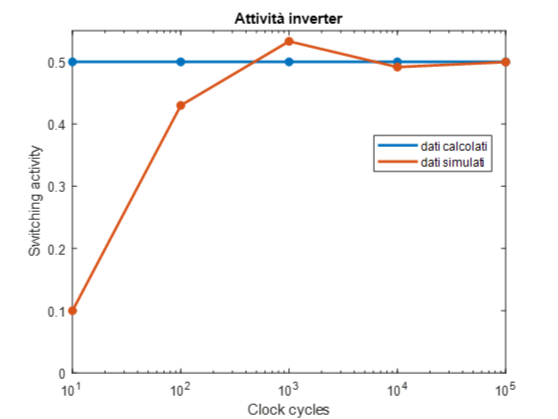
\includegraphics[width=7cm]{./img/Lab_1/Es_1/Inverter.png}%
        \label{fig:inv_sim}%
        }%
    \hfill%
    \subfloat[data b]{%
        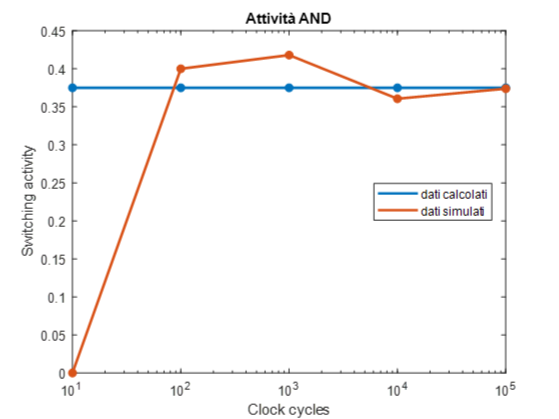
\includegraphics[width=7cm]{./img/Lab_1/Es_1/And.png}%
        \label{fig:and_sim}%
        }%
    \caption{all the data}
    \hfill
    \subfloat[data c]{%
        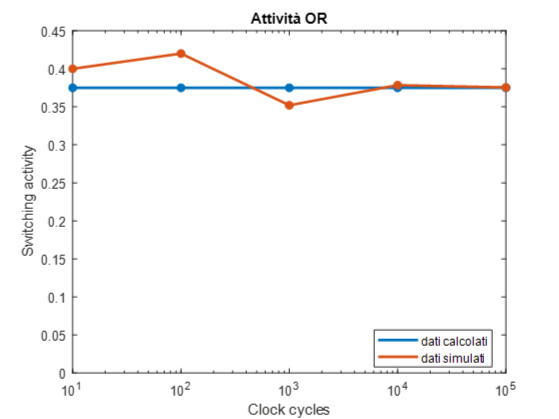
\includegraphics[width=7cm]{./img/Lab_1/Es_1/OR.png}%
        \label{fig:inv_sim}%
        }%
    \hfill%
    \subfloat[data d]{%
        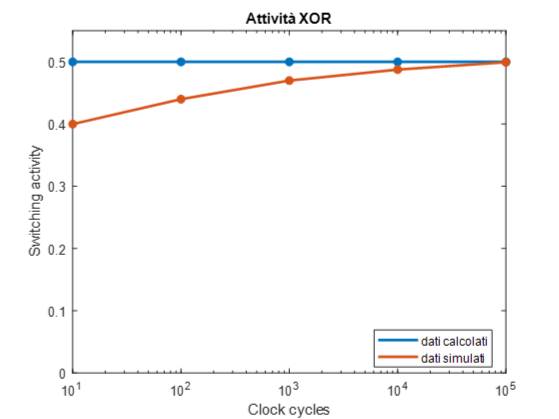
\includegraphics[width=7cm]{./img/Lab_1/Es_1/XOR.png}%
        \label{fig:and_sim}%
        }%
    \caption{all the data}
\end{figure}

Si osserva che all'aumentare del tempo di simulazione la stima della Esw risulta a man mano più accurata. In particolare, nel caso analizzato, si osserva che per un numero di cicli di clock superiore a 10000, i due dati sono confrontabili.


%%%%%%%%%%%%%%%%%%%%%%%%%%%%%%
%%%%%%%%%%%%%%%%%%%%%%%%%%%%%%
% chapter 2
\section{Calcolo di probabilit\`a e attivit\`a: half adder e full adder}

Dalle tavole di verità si ottengono le seguenti funzioni:

\begin{itemize}
\item \textbf{Half adder} \\
S = A XOR B
Cout = A AND B
\item \textbf{Full adder} \\
S = A XOR B XOR Cin
Cout = A AND B AND Cin
\end{itemize} 

Partendo dalle funzioni delle uscite è stato possibile ricavare le probabilità associate alle uscite e le relative switching activity.

\begin{itemize}
\item \textbf{Half adder} \\
P(S=1) = 
P(Cout = 1) =
A(S) =
A(COut) =
\item \textbf{Full adder} \\
P(S=1) = 
P(Cout = 1) =
A(S) =
A(COut) =
\end{itemize} 

Sfruttando i risultati ottenuti per il singolo full adder, è possibile ottenere le probabilità e le attività di un ripple carry adder di parallelismo 8 bit.
\\
schema
\\
Si considerano ingressi equiprobabili con eccezione del carry in ingresso al primo full adder, fissato a 0.\\
I risultati ottenuti sono riportati nella seguente tabella.

\begin{table}
\begin{center}
\begin{tabular}{|c|c|c|c|c|c|c|c|c|c|}
\hline
 & S7 & S6 & S5 & S4 \\
\hline
topolino & minni & tip & tap \\
\hline
\hline
paperino & paperina & orazio & clarabella \\
\hline
qui & quo & qua & ottoperotto \\
zio paperone & gastone & paperoga & battista \\ 
\hline 
\end{tabular}
\end{center}
\caption{A caption for your table}
\label{A-lable-for-your-table}
\end{table}

Variando le probabilità associate agli ingressi, in particolare considerando P(A=1) = 0.4 e P(B=1) = 0.6, si ottengono i seguenti risultati.

\begin{table}
\begin{center}
\begin{tabular}{|c|c|c|c|c|c|c|c|c|c|}
\hline
 & S7 & S6 & S5 & S4 \\
\hline
topolino & minni & tip & tap \\
\hline
\hline
paperino & paperina & orazio & clarabella \\
\hline
qui & quo & qua & ottoperotto \\
zio paperone & gastone & paperoga & battista \\ 
\hline 
\end{tabular}
\end{center}
\caption{A caption for your table}
\label{A-lable-for-your-table}
\end{table}

E' possibile notare come la probabilità delle varie uscite sia funzione delle probabilità degli ingressi.
I particolare, la probabilità delle uscite relative alle somme aumenta. Commenti su tabella

Al fine di avere un riscontro sui dati stimati, sono state effettuate due simulazioni tramite ModelSim: in un primo caso è stato considerato un ritardo solamente sulle uscite relative alla somme; successivamente è stato introdotto un ulteriore ritardo anche sul carry in uscita di ogni FA.
Come descritto precedentemente, il file fornito da Modelsim riporta il numero di commutazioni dei segnali, di conseguenza l'attività è stata calcolata come prima.

TABELLA ES 2 ANALISI

Si nota come la prima simulazione abbia fornito dati comparabili con quelli precedentemente stimati. Nella seconda simulazione, invece, la presenza di un ritardo sul carry di uscita di ogni FA ha come conseguenza un generale aumento dell'attività delle uscite di somma. Tale ritardo causa infatti glitch, responsabili dell'aumento della Esw.
Tale risultato è particolarmente evidente considerando la Esw totale dei due casi: si nota che la presenza del ritardo raddoppia tale valore.

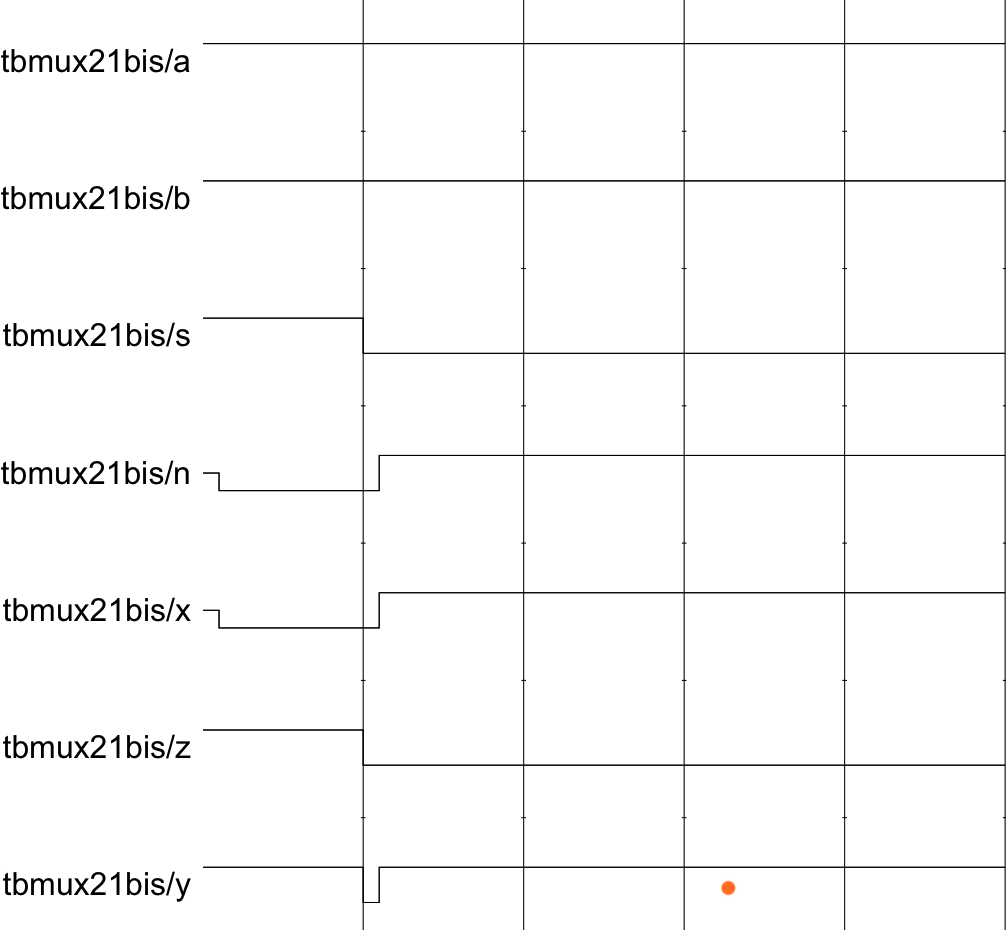
\includegraphics[width=6cm]{./img/Lab_1/Es_2/Glitch.png} 



\begin{itemize}
\item this is the first item
\item this is the second item...
\item if you want to change the point of the item do as in the following ite:
\item[-] whithin squared parentheses you can put a sign you like
\end{itemize} 


\subsection{Eample of an enumeration}

\begin{enumerate}
\item this is the first point
\item the second.....
\end{enumerate}



\subsection{example of a description}
\begin{description}
\item[latex] is a powerful editing and formatting language, whaich helps you
at writing reporte, books, letters, or whatever, just using the brain 
once at the beginning; it comes for free, and is completely portable
\item[word] is an awful terrible and nasty editing suite, it is proprietary,
not portable, it occupies a lot of space, you go mad with formatting,
and very often you loose you work all in a sudden. 
\end{description}


\subsection{Example of a table:}

\begin{table}
\begin{center}
\begin{tabular}{|c|c|c|c|}
\hline
pippo & pluto & indiana pipps & gilberto de pippis \\
\hline
topolino & minni & tip & tap \\
\hline
\hline
paperino & paperina & orazio & clarabella \\
\hline
qui & quo & qua & ottoperotto \\
zio paperone & gastone & paperoga & battista \\ 
\hline 
\end{tabular}
\end{center}
\caption{A caption for your table}
\label{A-lable-for-your-table}
\end{table}


Other features are available for table formatting: just refer to the manuals.
For what concerns equations: what do you think about the word equation editor?
Well, whatever you will try to do, you will loose your afternoom on it, and
still you are not sure it will have a decent aspect. The equation suite
in latex is extremely powerful, and her you anly a very small example:
refer to the manuals and to AMS-MATH suite for help.


\subsection{Example of a small equation:}

writing \\
an equation on line is easy $a \cdot \int^{\infty}_0 i(t)
\frac{di}{dt}$
while if you want to better display it just include it in this way:
$$a \cdot \int^{\infty}_0 i(t) \frac{di}{dt}$$

and finally if you want to refer and number the equation as the
\ref{label-my-equation} then the syntax is:

\begin{equation}
a \cdot \int^{\infty}_0 i(t) \cdot \frac{di}{dt}
\label{label-my-equation}
\end{equation}
%%%%%%%%%%%%%%%%%%%%%%%%%%%%%%
%%%%%%%%%%%%%%%%%%%%%%%%%%%%%%

% chapter 4
\section{Analisi di un Multiplexer}


% include here only file for the third lesson and homeworks
% here the path to figures and VHDL should be ./exe3/

\section{Analisi di un Contatore Sincrono}

